\chapter{Demonstrator Applikation}
\label{Kap5}
\label{chap:Kap5}
Als praktischer Teil dieser Arbeit wurde das Netzwerk basierte System implementiert. Mit der Applikation können zwei Anwender auf Endgeräten gespeicherte Fotos auswählen und durch einen Bump übertragen.

Die Implementierung wurde auf der iOS Plattform in der Programmiersprache Swift durchgeführt und ist als Git Repository erreichbar unter:

\url{https://github.com/informatik-mannheim/thesis-bump-to-transfer/tree/master/sources/Bumper}

Für das User-Interface der Applikation wurde ein Wireframe erstellt, das als PDF aufzufinden ist unter:

\url{https://github.com/informatik-mannheim/thesis-bump-to-transfer/blob/master/sources/Wireframe.pdf}

Folgend wird das Wireframe in Auszügen dargestellt um einen Einstieg in die Nutzung der Applikation zu bieten. Auf den Screenshots ist sichtbar welche Interaktionsmöglichkeiten dem Anwender, vor und nach der Durchführung der Interaktion, geboten werden. Von besonderem Interesse ist dabei zum einen wie der Anwender gespeicherten Inhalte durchsuchen und für den Versand auswählen kann und zum anderen wie empfangene Daten angezeigt und gespeichert werden können.

\subsubsection{}
\begin{figure}[H]
  \centering
  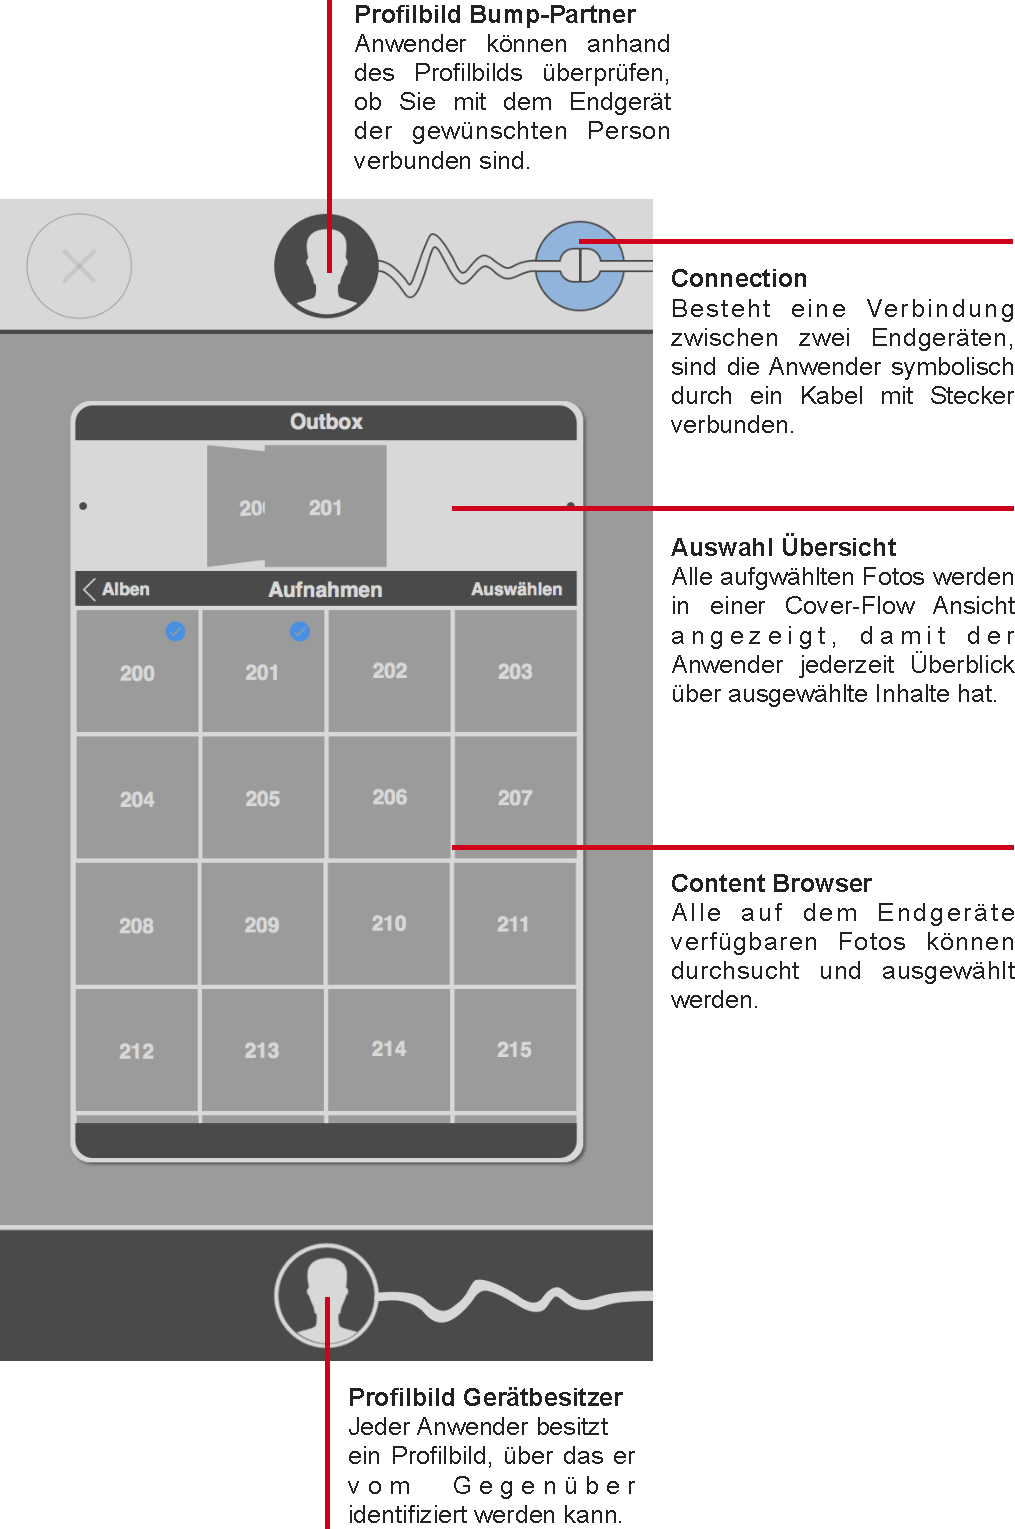
\includegraphics[width=\linewidth]{kapitel5/wireframe1.pdf}
\end{figure}

\subsubsection{}
\begin{figure}[H]
  \centering
  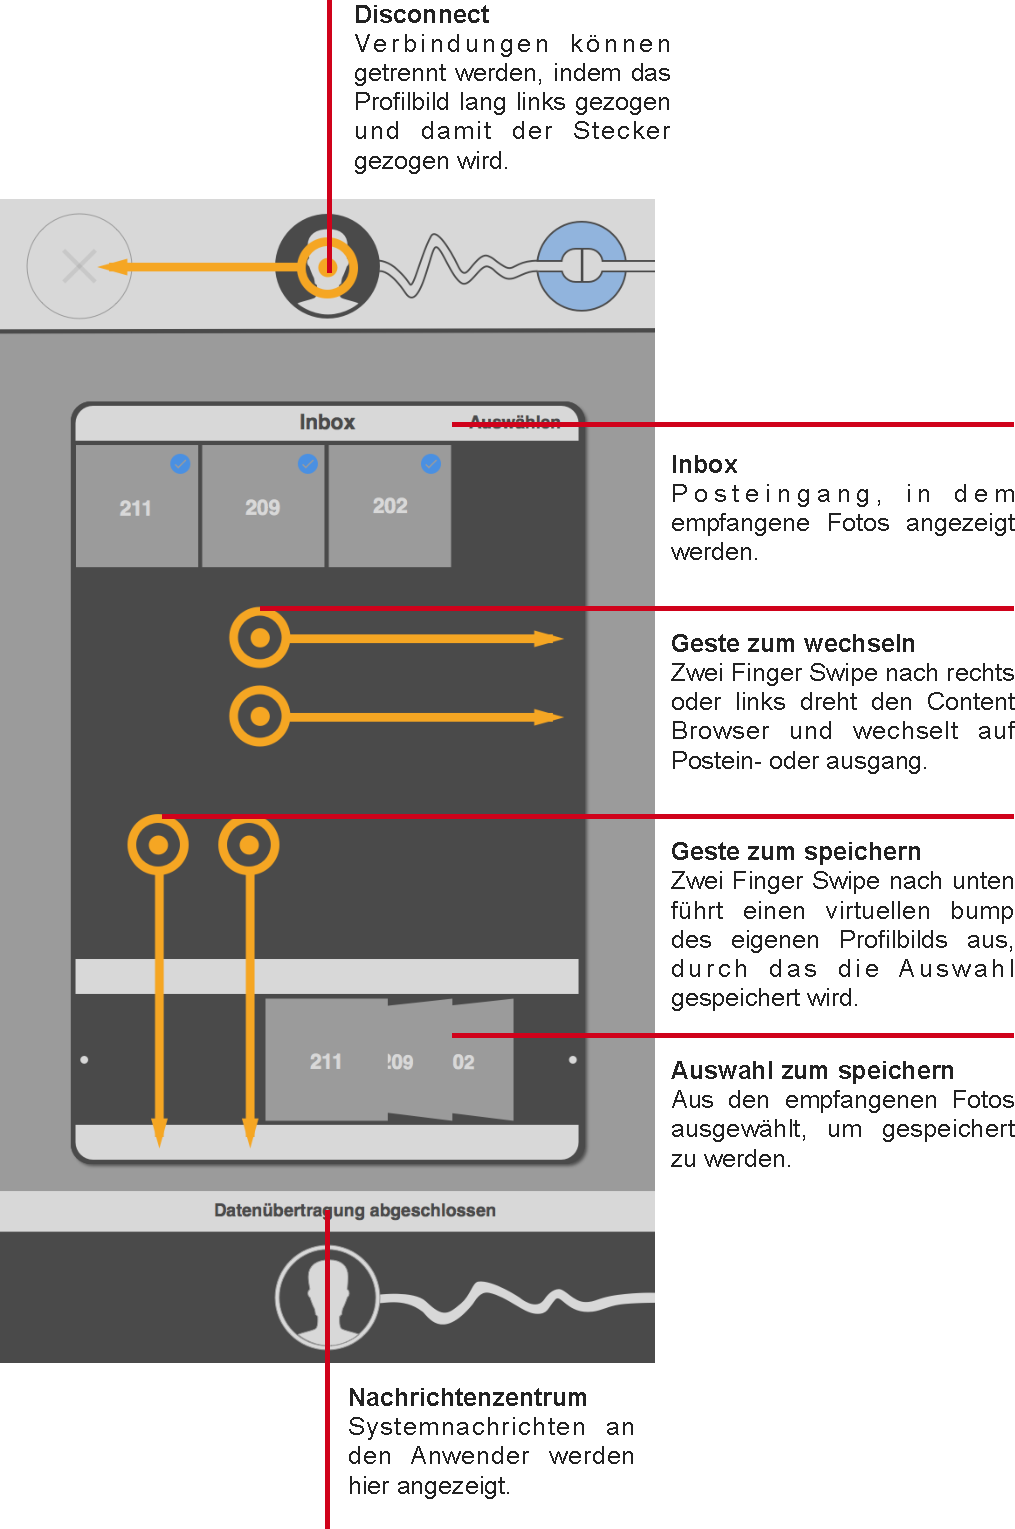
\includegraphics[width=\linewidth]{kapitel5/wireframe2.pdf}
\end{figure}